\documentclass{beamer}

\usepackage{booktabs}
\usepackage{color}
\usepackage{graphicx}
\usepackage[backend=bibtex]{biblatex}

\title[Curricula and LDA]{Unsupervised academic curricula evaluation
  through Latent Dirichlet allocation}
\author{Jean Michel Rouly \and Huzefa Rangwala}
\date{Updated \today}

\usetheme{Boadilla}
\usecolortheme{rose}

\bibliography{../bibliography/bibliography.bib}

\begin{document}

  \frame{\titlepage}

  \begin{frame}{Research goal}

  \vfill

  Through the application of probabilistic machine learning methods,
  specifically LDA topic modeling, a corpus of unstructured course
  descriptions can be digested and mined for topics. In this scenario, each
  topic represents a core concept covered by the courses.

  \vfill

  A research framework will be constructed to read data from the
  Internet, digest into a common internal format, pipeline into an LDA
  topic model, and ultimately visualize in an interactive manner.

  \vfill

  Ultimately the automatically discovered topics can be used in
  end-user university evaluation processes.

  \vfill

\end{frame}


  \begin{frame}{Motivation}

  \begin{itemize}
    \item University course data widely available online.
    \item Human-readable course descriptions detail what concepts are taught.
    \item \textbf{Human-readable} course descriptions require manual inspection.
  \end{itemize}


%  \onslide<+->
%  \begin{block}{Program of study}
%    A defined, ordered set of courses at a university with the goal of
%    achieving a degree, certification, etc.
%  \end{block}
%
%  \onslide<+->
%  \begin{block}{Course}
%    A set of learning outcomes and techniques to achieve them, defined by
%    a syllabus.
%  \end{block}
%
%  \onslide<+->
%  \begin{block}{Syllabus}
%    Unstructured collection of keywords and phrases that describes the
%    core concepts and outcomes of a specific course.
%  \end{block}

\end{frame}


  \begin{frame}{Background information}

  \onslide<+->
  \begin{block}{Machine Learning}
    Interdisciplinary field combining
    elements of Artificial Intelligence and Statistics that allows
    programs to approximate unknown functions based on complex datasets.
  \end{block}

  \onslide<+->
  \begin{block}{Latent Variable Modeling}
    Subfield of Machine Learning that focuses on reconstructing
    ``hidden'' or unobservable variables that influence the structure of
    a dataset.
  \end{block}

  \onslide<+->
  \begin{block}{Topic Modeling}
    Example of latent variable modeling that discovers \alert{topics}
    that occur in a dataset.
  \end{block}

  \onslide<+->
  \begin{block}{Latent Dirichlet allocation}
    Generative approach to topic modeling, starts with unknown variables
    and \emph{generates} documents.
  \end{block}
\end{frame}


%  \begin{frame}{Latent Dirichlet allocation}

  \only<1>{
    \begin{figure}
      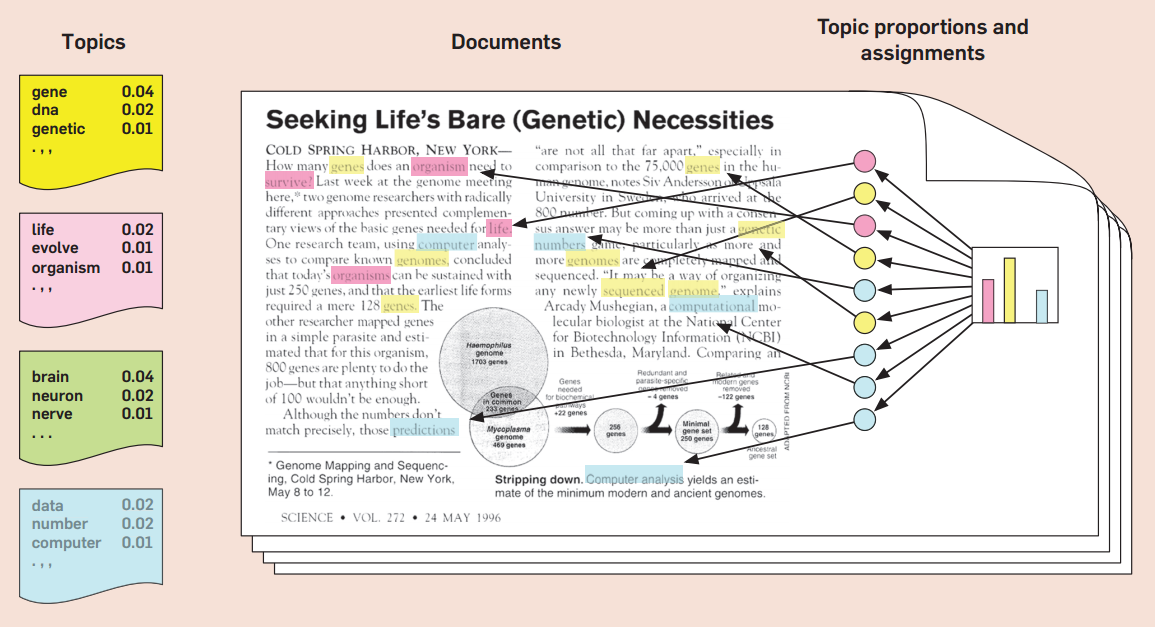
\includegraphics[width=0.8\framewidth]{figs/blei-lda.png}
      \caption{The LDA generative model.\footfullcite{Blei2012}}
    \end{figure}
  }

  \only<2>{
    \begin{align*}
      p(\beta_{1:K}, \theta_{1:D},z_{1:D} | w_{1:D}) = \frac{\beta_{1:K},
      \theta_{1:D},z_{1:D}, w_{1:D}}{w_{1:D}}
    \end{align*}

    \vfill

    Gibbs sampling is used to approximate the probability of the
    denominator (evidence)\footfullcite{Blei2012}.

    \vfill

    \begin{itemize}
      \item $\beta_{1:k} := \text{ topic } k$
      \item $\theta_{d,k} := \text{ topic proportion for topic } k \text{
      in document } d$
      \item $z_{d,n} := \text{ topic assignment for word } n \text{ in
      document } d$
      \item $w_{d,n} := \text{ the } n^{th} \text{ word in document } d$
    \end{itemize}
  }

\end{frame}


  \begin{frame}{Progress so far}
    \begin{itemize}
      \item Collect preliminary course description dataset.
      \item Perform exploratory clustering.
      \item Expand initial prototype to include LDA computation.
      \item Build preliminary visualization tool.
      \item Run LDA experiments varying initialization parameters.
      \item Construct course prerequisite trees.
      \item Implement metrics for department/course comparison.
    \end{itemize}
  \end{frame}

  \begin{frame}{Framework}

  \begin{block}{Scrape}
    Modular Python command line application that supports custom input
    data sources (syllabus archives) \& multiple clustering tools.
    Pluggable backend scraping engines contribute to flexibility. Defines
    \texttt{export}/\texttt{import} utility for interfacing with the
    \texttt{Learn} module.
  \end{block}

  \vfill

  \begin{block}{Learn}
    Java program that adaptively ingests data generated by the scrape
    module. Makes heavy use of MALLET to perform LDA.
  \end{block}

  \vfill

  Open source and available at:\\
  \url{https://github.com/jrouly/trajectory}\\
  \url{http://leo.cs.gmu.edu/svn/users/jrouly/trajectory}

\end{frame}


  \begin{frame}{Resources}

  \only<1>{
    \framesubtitle{Software Toolkits}

    \begin{block}{\texttt{SQLAlchemy}}
      High level database model abstractions for a pluggable, easy to use
      database layer. \\ \url{http://sqlalchemy.org}
    \end{block}

    \begin{block}{MALLET}
    ``MALLET is a Java-based package for statistical natural language
    processing, document classification, clustering, topic modeling,
    information extraction, and other machine learning applications to
    text.'' \\ \url{http://mallet.cs.umass.edu}
    \end{block}

    \begin{block}{\texttt{BeautifulSoup}}
      Efficient and easy to use Web scraping and HTML manipulation
      library. \\
      \url{http://www.crummy.com/software/BeautifulSoup}
    \end{block}
  }

  \only<2>{
    \framesubtitle{Course Description Data}

    Data collected from Computer Science departments at various
    universities.

    \vfill

    Current institutions represented:

    \begin{itemize}
      \item George Mason University
      \item Louisiana State University
      \item Kansas State University
      \item Portland State University
      \item Rensselaer Polytechnic Institute
      \item Stanford University
    \end{itemize}

    (primarily because they offer easily-accessed public course catalogs).

  }

\end{frame}


%  \begin{frame}{Preliminary results}

  \only<1>{
    \framesubtitle{Clustering}
    \begin{block}{Data}
      \begin{itemize}
        \item Scraped from \url{http://cs.gmu.edu/syllabus} archive.
        \item 1369 syllabus files, some empty.
        \item 1268 data rows (non-zero syllabi), 7189 features (terms).
        \item 292 categories (unique section numbers).
      \end{itemize}
    \end{block}

    \begin{table}
      \centering
      \begin{tabular}{ll}
      \toprule
      Execution time & 0.144568s \\
      Homogeneity & 0.415 \\
      Completeness & 0.877 \\
      \bottomrule
      \end{tabular}
      \caption{Preliminary clustering metrics\label{table:metrics}}
    \end{table}
  }

  \only<2>{
    \framesubtitle{Clustering}
    \begin{table}
      \centering
      \begin{tabular}{llll}
      \toprule
      Cluster 1 &
      Cluster 2 &
      Cluster 3 &
      Cluster 4 \\
      \midrule
      intelligence & chapter      & software     & operating \\
      artificial   & project      & swe          & systems \\
      agents       & sipser       & testing      & projects \\
      learning     & networks     & web          & aydin \\
      tecuci       & layer        & interfaces   & synchronization \\
      expert       & savitch      & construction & scheduling \\
      knowledge    & data         & design       & homeworks \\
      reasoning    & dlc          & constructing & processes \\
      semantic     & experimental & professor    & group \\
      intelligent  & design       & quality      & friday \\
      \bottomrule
      \end{tabular}
      \caption{10 Most frequent terms in first four clusters\label{table:results}}
    \end{table}
  }

  \only<3>{
    \framesubtitle{Topic Modeling: Documents}
    \begin{table}[ht]
    \centering
    \begin{tabular}{ll}
    \toprule
    Max Tokens: & 12715 \\
    Total Tokens: & 588131 \\
    Total Syllabi: & 1570 \\
    Size on Disk: & 9.1MB clean, 113MB raw \\
    \bottomrule
    \end{tabular}
    \end{table}

    \vfill

    \begin{table}[ht]
    \centering
    \begin{tabular}{lllll}
    \toprule
    Doc & Topic & Proportion & Topic & Proportion \\
    \midrule
    0 & 33 & 0.7666641741676518 & 62 & 0.230550274742815 \\
    1 & 44 & 0.5776374037067855 & 8  & 0.3152509716025131 \\
    2 & 86 & 0.8143297134325639 & 62 & 0.18015768047706127 \\
    3 & 9  & 0.9491106700671812 & 5  & 0.034876914241398584 \\
    4 & 82 & 0.5736690412365056 & 53 & 0.39539480434234386 \\
    \bottomrule
    \end{tabular}
    \caption{First five documents and their top two topics\label{table:ldadocs}}
    \end{table}
  }

  \only<4>{
    \framesubtitle{Topic Modeling: Topics}
    \begin{table}[ht]
    \centering
    \begin{tabular}{llll}
    \toprule
    Topic & Term & Term & Term \\
    \midrule
    0 & lisp (98)          & june (57)        & prolog (46)    \\
    1 & systems (154)      & operating (119)  & system (101)   \\
    2 & systems (304)      & operating (252)  & students (189) \\
    3 & randomization (66) & trials (57)      & clinical (57)  \\
    4 & database (389)     & relational (151) & design (133)   \\
    \bottomrule
    \end{tabular}
    \caption{First five topics and their top four terms\label{table:ldatopics}}
    \end{table}
  }

\end{frame}


  \begin{frame}{Visualization tool}

    \begin{itemize}
      \item Interactive browser-based application.
      \item Allows both high level overview of dataset and low level view of per-course topic inferences.
      \item Provides view of
        \begin{itemize}
          \item topics
          \item departmental comparison
          \item prerequisite chains
          \item dataset dashboard
        \end{itemize}
    \end{itemize}
  \end{frame}

%  \begin{frame}{Proposed visualization tool}
%
%    \only<1>{
%      \begin{itemize}
%        \item Import results of the LDA function back into the database
%          layer, possibly with pedigree data (ie.\ knowledge of which run
%          what data came from) Link it all up back to the existing scraped
%          meta information.
%        \item Host the database as a backend to a simple responsive
%          user-facing browser-based web application.
%        \item Feature: visualization of data, possibly graph-based.
%        \item Feature: query interface allowing user to search through
%          mined and inferred data sources.
%      \end{itemize}
%    }
%
%  \end{frame}

%  \begin{frame}{Continued development goals}

  Ultimately: visualization \& comparison of university programs of study
  given unknown dataset of course descriptions.

  \begin{description}
    {\color{green}\item[Metadata awareness] Track information like course number,
      semester, institutional information, etc.}
    \item[Prerequisite chains] Use metadata to track lists of
    prerequisite courses.
    \item[Rich visualizations] Investigate use of
    D3.js\footnote{\url{http://d3js.org}} to develop rich, visually
    pleasing, interactive tools.
    \item[Evaluation suite] Correlate results against existing third
    party evaluations, manual inspection, other instutitions.
  \end{description}

\end{frame}


%  \begin{frame}
%  \begin{center}
%  \Huge Questions?
%  \end{center}
%  \end{frame}

\end{document}
